\documentclass[10pt, twocolumn]{article}

\usepackage[margin=0.75in]{geometry}
\usepackage{amsmath,amsthm,amssymb,bm}
\usepackage{xcolor}
\usepackage{cancel}
\usepackage{graphicx}
\usepackage{changepage}
\usepackage{circuitikz}
\usepackage{pgfplots}
\usepackage{minted}
\usepackage{physics}
\usepackage{tikz}
\usepackage{tikz-3dplot}
\usepackage{hyperref}
\usepackage{cleveref}
\usepackage[uncertainty-mode = separate, separate-uncertainty-units = single]{siunitx}
\usepackage{fontspec}
\usepackage{relsize}
\usepackage{subcaption}
\usepackage{todonotes}
\usepackage{multicol, multirow, booktabs}
\usepackage[breakable]{tcolorbox}
\usepackage[inline]{enumitem}

\theoremstyle{definition}
\newtheorem{problem}{Problem}
\newtheorem{soln}{Solution}

\pgfplotsset{compat=newest}
\usetikzlibrary{lindenmayersystems}
\usetikzlibrary{arrows}
\usetikzlibrary{calc}
\usetikzlibrary{positioning, fit}
\usetikzlibrary{3d, perspective}
\usetikzlibrary{math}
\usetikzlibrary{fadings}
\usetikzlibrary{angles,quotes} 

\definecolor{incolor}{HTML}{303F9F}
\definecolor{outcolor}{HTML}{D84315}
\definecolor{cellborder}{HTML}{CFCFCF}
\definecolor{cellbackground}{HTML}{F7F7F7}
\newcommand{\bv}[1]{\bm{\mathrm{#1}}}
\newcommand{\ui}{\bv{\hat{i}}}
\newcommand{\uj}{\bv{\hat{j}}}
\newcommand{\uk}{\bv{\hat{k}}}
\newcommand{\ux}{\bv{\hat{x}}}
\newcommand{\uy}{\bv{\hat{y}}}
\newcommand{\uz}{\bv{\hat{z}}}
\newcommand{\uv}[1]{\hat{\bv{{#1}}}}
\newcommand{\pd}[2][]{{\frac{\partial^{#1}}{\partial {{#2}^{#1}}}}}
\newcommand{\dif}[2][]{{\frac{d^{#1}}{d{{#2}^{#1}}}}}
\newcommand{\grd}{\nabla}

\pgfdeclarelayer{background}  
\pgfsetlayers{background,main}
\AtBeginDocument{\RenewCommandCopy\qty\SI}

\makeatletter
\newcommand{\boxspacing}{\kern\kvtcb@left@rule\kern\kvtcb@boxsep}
\makeatother
\newcommand{\prompt}[4]{
    \ttfamily\llap{{\color{#2}[#3]:\hspace{3pt}#4}}\vspace{-\baselineskip}
}

\newcommand{\thevenin}[2]{
  \begin{center}
    \begin{circuitikz} \draw
      (0,0) -- (2,0) to[battery1, l_=$V_{Th}\eq#1$] (2,2) 
      to[resistor, l_=$R_{Th}\eq#2$] (0,2)
      ;
      \draw [o-] (-.07,2.079);
      \draw [o-] (-.07,0.079);
    \end{circuitikz}
  \end{center}
}

\newcommand{\norton}[2]{
  \begin{center}
    \begin{circuitikz} \draw
      (0,0) -- (3,0) to[american current source, l_=$I_{N}\eq#1$] (3,2) -- (0,2) (2,0)
      to[resistor, l=$R_{N}\eq#2$] (2,2)
      ;
      \draw [o-] (-.07,2.079);
      \draw [o-] (-.07,0.079);
    \end{circuitikz}
  \end{center}
}

\DeclareMathOperator{\Div}{div}
\DeclareMathOperator{\Curl}{curl}
\DeclareMathOperator{\sgn}{sgn}

\newcommand{\highlight}[1]{\colorbox{yellow}{$\displaystyle #1$}}

\newcommand{\ti}[1]{\widetilde{#1}}

\newfontface{\Kaufmann}{Kaufmann}
\DeclareTextFontCommand{\kf}{\Kaufmann}
\newcommand{\scriptr}{\fontsize{12pt}{12pt}\kf{r}\fontsize{10pt}{10pt}}

\newfontface{\KaufmannB}{Kaufmann Bold}
\DeclareTextFontCommand{\kfb}{\KaufmannB}
\newcommand{\bscriptr}{\fontsize{12pt}{12pt}\kfb{r}\fontsize{10pt}{10pt}}
\newcommand{\justif}[2]{&{#1}&\text{#2}}

\title{Math 3160H: Special Function Report - Expansion of Electromagnetic Potential}
\author{Jeremy Favro (0805980) \\ Trent University, Peterborough, ON, Canada}
\date{\today}

\begin{document}
\maketitle
\todo{Define all the r' stuff etc.}
\section{Electrostatics \& the Steady State Potential}
\subsection{Motivation}
A common (really the only) problem in electro\emph{statics} \todo{How to glossary} is finding the electric field of some stationary charge distribution.
This is accomplished by Coulombs law,
\begin{equation}
  \bv{E}(\bv{r})=\frac{1}{4\pi\epsilon_0}\int \frac{\uv{\bscriptr}}{\scriptr} \rho(\bv{r}')dr\tau'.
  \label{eqn:e-field-integral}
\end{equation}
\todo{\scriptr}
This integral becomes complicated quickly for nontrivial charge distributions. When these more complex situations arise we can still use
\emph{Gauss' law} if the charge distribution has some kind of exploitable symmetry, but these situations are rare. Instead we seek a potential,
\begin{equation}
  V(\bv{r})=\frac{1}{4\pi\epsilon_0}\int\frac{1}{\scriptr}\rho(\bv{r}')d\tau'.
  \label{eqn:potential-integral}
\end{equation}
But this integral is still sometimes too hard! $\rho(\bv{r}')$, the volume charge density, is also often unknown in real situations.  Instead we use the time
independent form of the first Maxwell equation, $\bv{\nabla}\cdot \bv{E}=\rho/\epsilon_0$, along with the fact that our definition of the potential is that
$\bv{E}=-\bv{\nabla}V$, to show that
\begin{equation}
  \bv{\nabla}\cdot \bv{E}=-\nabla^2V=\frac{\rho}{\epsilon_0}
  \label{eqn:poisson}
\end{equation}
also known as \emph{Poisson's equation}. Note that to even define such a potential we require that $\bv{\nabla}\times\bv{E}=0$ (the second Maxwell equation),
which we will see later is not always true! Often we can work our problems such that we are actually interested in solving for $V$ in a region
where $\rho=0$ (though $\rho$ identically zero would imply $V$ identically zero), and so \cref{eqn:poisson} becomes
\begin{equation}
  \nabla^2 V=0,
  \label{eqn:laplace}
\end{equation}
\emph{Laplace's equation}.

\subsection{The Static Potential}
There are many ways of solving Laplace's equation, but since we are interested specifically in the expansion of the electric potential,
we will take the approach of a \emph{multipole expansion}. Consider some arbitrary charge distribution. If you are very far from the charges, their
potential $V$ and electric field $\bv{E}$ will look like those of point charges, just like how if you are very distant from Earth, its gravitational field
becomes that of a point mass, with none of the unevenness of the real Earth due to density changes \todo{Grav map of earth} (classical gravitation and
electrostatics have much in common in this way). The potential due to a point charge $Q$ is easily found by \cref{eqn:potential-integral} to be
\begin{equation}
  V=\frac{1}{4\pi \epsilon_0} \frac{Q}{r}.
  \label{eqn:point-potential}
\end{equation}
but what if $Q=0$? Not necessarily that there is no charge, but that there is no \emph{net charge}, like the case of the Hydrogen atom; one electron of charge
$-e$ and one proton of charge $+e$. Should this configuration produce $V=0$ everywhere? This greatly limits the usefulness of the potential if so! Consider
a \emph{physical electric dipole},
\begin{center}
  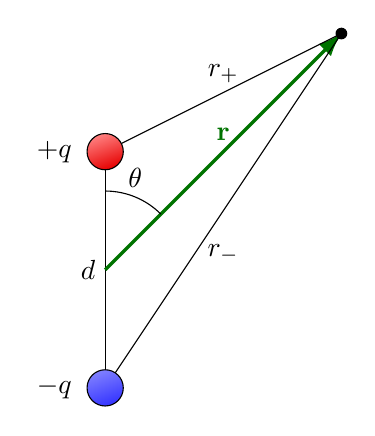
\begin{tikzpicture}
    \colorlet{Ecol}{orange!90!black}
    \colorlet{EcolFL}{orange!80!black}
    \colorlet{FCol}{red!60!black}

    \colorlet{veccol}{green!45!black}
    \tikzstyle{charge+}=[thin,top color=red!50,bottom color=red!90!black,shading angle=20]
    \tikzstyle{charge-}=[thin,top color=blue!50,bottom color=blue!80,shading angle=20]
    \tikzstyle{charge0}=[very thin,top color=green!80!black!50,bottom color=green!80!black,shading angle=20]

    \tikzstyle{O}=[top color=red!60,bottom color=red!90!black,shading angle=10]
    \tikzstyle{H}=[top color=white,bottom color=white!90!black,shading angle=10]
    \tikzstyle{vector}=[-Latex,very thick,veccol]



    \def\R{0.23}
    \def\d{3.0}
    \def\h{0.7}
    \coordinate (R) at (\d, \d);
    \coordinate (O) at (0,0);
    \coordinate (Q-) at (0,-\d/2);
    \coordinate (Q+) at (0,+\d/2);

    % CONNECTOR
    \draw (Q-) -- (Q+) node[midway, left] {$d$};

    % POSITION VECTOR
    \draw[vector] (O) -- (R) node[midway, above]{$\bv{r}$};
    \draw[] (Q+) -- (R) node[midway, above]{$\scriptr_+$};
    \draw[] (Q-) -- (R) node[midway, below=0.3cm]{$\scriptr_-$};
    \draw (O) ++(0,1) arc (90:45:1) node[midway, above]{$\theta$};
    \node at (R) [circle,fill,inner sep=1.5pt]{};

    % CHARGES
    \draw[charge-] (Q-) circle (\R) node[scale=1.0, left=0.3cm] {$-q$};
    \draw[charge+] (Q+) circle (\R) node[scale=1.0, left=0.3cm] {$+q$};
  \end{tikzpicture}
\end{center}
We know the potential due to $\pm q$ to be
$$V_\pm(\bv{r})=\frac{1}{4\pi \epsilon_0}\frac{\pm q}{\scriptr_\pm}$$
and since potential obeys \emph{linear superposition} the total potential is given by
$$V_\pm(\bv{r})=\frac{q}{4\pi \epsilon_0}\left[\frac{1}{\scriptr_+}-\frac{1}{\scriptr_-}\right].$$
From the cosine law we can write
$$\scriptr_\pm^2=r^2+(d/2)^2\mp rd\cos\theta=r^2\left(1\mp\frac{d}{r}\cos\theta+\frac{d^2}{4r^2}\right)$$
and since we are interested in the $r\gg d$ approximation the third term is negligible. Hence
$$\frac{1}{\scriptr_\pm}\approx\frac{1}{r}\left(1\mp \frac{d}{r}\cos\theta\right)^{-1/2}\approx \frac{1}{r}\left(1\pm\frac{d}{2r}\cos\theta\right)$$
using the binomial approximation. Hence
$$\frac{1}{\scriptr_+}-\frac{1}{\scriptr_-}\approx \frac{d}{r^2}\cos\theta,$$
and so
$$V(\bv{r})\approx \frac{1}{4\pi\epsilon_0}\frac{qd\cos\theta}{r^2}.$$
As we expected, this decays like $1/r^2$ and so is nearly zero at large $r$. We can extend this to larger charge distributions by tacking on additional dipoles
which invites the development of some way to expand any \emph{compact} charge distribution in this way. \todo{Blob figure here (3.28)}
We know that the potential is given in general by \cref{eqn:potential-integral}. Using the cosine law again we see that
$$\scriptr^2=r^2+r'^2-2rr'\cos\alpha=r^2\left[1+\left(\frac{r'}{r}\right)^2-2\frac{r'}{r}\cos\alpha\right],$$
where $\alpha$ is the angle between $\bv{r}$ and $\bv{r}'$. We can hence say that
$$\frac{1}{\scriptr} = \frac{1}{r\sqrt{1+\left(\frac{r'}{r}\right)^2-2\frac{r'}{r}\cos\alpha}}.$$
Which, since we know we're looking for a special function expansion (otherwise this can be seen by Taylor expansion of the resultant binomial),
looks a lot like the generating function for the Legendre polynomials,
\begin{equation}
  \frac{1}{\sqrt{1-2xt+t^2}}=\sum_{n=0}^\infty t^nP_n(x)
  \label{eqn:legendre-generating}
\end{equation}
where $x=\cos\alpha$ and $t=\frac{r'}{r}$. Indeed,
$$
  \frac{1}{\scriptr}=\frac{1}{r}\sum_{n=0}^\infty\left(\frac{r'}{r}\right)^nP_n(\cos\alpha)
$$
and hence
\begin{equation}
  V(\bv{r})=\frac{1}{4\pi\epsilon_0}\sum_{n=0}^\infty\frac{1}{r^{n+1}}\int (r')^nP_n(\cos\alpha)\rho(\bv{r}')d\tau'
  \label{eqn:multipole-expansion-potential}
\end{equation}
where, if we orient our coordinate system so that $\bv{r}$ lies along $\uz$, $\alpha$ becomes the polar angle $\theta'$ in spherical-polar coordinates.
This is the multipole expansion! It allows us to much more easily calculate an approximate potential at large distances since the Legendre polynomials are not hard
to integrate and if greater precision is required, we can just do more integrals!
\todo{Maybe comment further on dipoles, plot potentials}
% \begin{tikzpicture}
%   \begin{axis}[
%       colormap/jet,
%       colorbar,
%       view={0}{90}]
%     \addplot3[surf, shader=flat] {1/sqrt(x^2+(y+1/2)^2)-1/sqrt(x^2+(y-1/2)^2)};
%   \end{axis}
% \end{tikzpicture}
\subsection{Moving Charges \& Magnetostatics}
Everything we did above assumed that the charge distributions were \emph{static} (though the test points needed not be).
When things start to move, fields other than $\bv{E}$ arise. Unlike in mathematics classes, there is no hint that these new fields
would arise from previous static situations. A lot of experimental work was done to create a model for the magnetic field after
physicist Hans Christian Oersted discovered, in 1820, that when he moved a compass near a wire the needle would turn when electric \emph{current} passed through the wire.

Naively, one might think that this is somehow due to the current (which, awkwardly, is defined as if positive charges were its origin) creating a
charge buildup in the wire which attracts the compass needle. This doesn't work as an explanation as a test charge placed near the wire would experience
no force! \todo{I'm lying. Problem 7.45.} This is because, even though electrons are flowing along the wire, there are just as many (fixed) positive charges (protons)
as there are moving negative charges.

Okay, so there's something going on here other than an electric field. We call this new field the \emph{magnetic field}, $\bv{B}$. It is produced
by charges (positive or negative) in motion. I could give more prose here but since we just want to get to the potential and start trying to expand
it, we'll just come out and say the next two Maxwell equations:
\begin{align}
  \bv{\nabla}\cdot\bv{B}  & =0 \label{eqn:divB} \\
  \bv{\nabla}\times\bv{B} & =\mu_0\bv{J}
  \label{eqn:curlB}
\end{align}
where $\bv{J}$ is the \emph{volume current}, the amount of charge passing through a volume per a time. As usual there are many ways to actually
find the magnetic field. One of the most general is the \emph{Biot-Savart law},
\begin{equation}
  \bv{B}(\bv{r})=\frac{\mu_0}{4\pi}\int \frac{\bv{J}(\bv{r}')\times \uv{\bscriptr}}{\scriptr^2}.
  \label{eqn:biot-savart}
\end{equation}
This ``law'' only holds for nonrelativistic ($v\ll c$) charges and for steady state currents. Again though we run into the problem
that this integral can get \emph{hard} to calculate. There are of course other approaches to finding the field, similar to how we could use
Gauss' law in electrostatics when there was exploitable symmetry, in magnetostatics we can sometimes use the integral form of \cref{eqn:curlB},
\begin{equation}
  \oint \bv{B}\cdot d\bv{\ell}=\mu_0 I_{enc}
  \label{eqn:amperes-law}
\end{equation}
where we are integrating around an \emph{Amp\`erian loop} enclosing total current $I_{enc}$. But again this is only applicable in situations
of high symmetry! So what do we do? Introduce another potential! In electrostatics we had that $\bv{\nabla}\times\bv{E}=0$ let us introduce a
scalar potential $V$ such that $\bv{E}=-\bv{\nabla}V$. Unfortunately since \cref{eqn:curlB} says $\bv{B}$ isn't a conservative field,
we can't define a scalar potential. We do however have \cref{eqn:divB} which invites the definition of a \emph{vector} potential $\bv{A}$ such
that
\begin{equation}
  \bv{B}=\bv{\nabla}\times \bv{A}.
  \label{eqn:vec-pot}
\end{equation}
Let's see how this works out with the Maxwell equations for $\bv{B}$. \cref{eqn:divB} is covered, since the divergence of a curl is always zero. 
\cref{eqn:curlB} becomes 
$$\bv{\nabla}\times\bv{B}=\bv{\nabla}\times(\bv{\nabla}\times \bv{A})=\bv{\nabla}(\bv{\nabla}\cdot \bv{A})-\nabla^2\bv{A}=\mu_0\bv{J}.$$
Now, just as the electrostatic potential was defined only up to addition of an object whose divergence was zero (a constant), 
the magnetic vector potential is only defined up to addition of an object whose curl is zero, which will have no effect on $\bv{B}$.
This allows us to set $\bv{\nabla}\cdot\bv{A}=0$. You can prove this but it is not particularly enlightening here so I will omit it.
With this change we can say that 
$$
\nabla^2\bv{A}=-\mu_0\bv{J},
$$
Poisson's equation again, actually three of them - one for each cartesian coordinate. For a $\bv{J}$ that vanishes at infinity then 
\begin{equation}
  \bv{A}(\bv{r})=\frac{\mu_0}{4\pi}\int \frac{\bv{J}(\bv{r}')}{\scriptr}d\tau'.
  \label{eqn:vec-pot-integral}
\end{equation}
This definition gives up a similar expansion as to what we had done previously. Recall we found by way of cosine law that 
$$\frac{1}{\scriptr}=\frac{1}{\sqrt{r^2+r'^2-2rr'\cos\alpha}}=\frac{1}{r}\sum_{n=0}^{\infty}\left(\frac{r'}{r}\right)^nP_n(\cos\alpha)$$
where $\alpha$ is the angle between $\bv{r}$ and $\bv{r}'$. This lets us rewrite \cref{eqn:vec-pot-integral} as
\begin{align}
  \bv{A}(\bv{r})&=\frac{\mu_0I}{4\pi}\oint \frac{1}{\scriptr}d\bv{\ell}'=\frac{\mu_0I}{4\pi}\int_{n=0}^{\infty}\frac{1}{r^{n+1}}\oint (r')^nP_n(\cos\alpha)d\bv{\ell}'\nonumber\\
  &=\frac{\mu_0I}{4\pi}\left[\frac{1}{r}\oint d\bv{\ell}'+\frac{1}{r^2}\oint r'\cos\alpha d\bv{\ell}'+\dots\right].
\end{align}
Note that the first term is the displacement around an entire curve, zero. This is no accident. It arises as a consequence of 
$\bv{\nabla}\cdot\bv{B}=0$ and the assumption that there are no magnetic monopoles. This is (or was) an area of intense
experimental research. Much work has been done to try to observe a magnetic monopole but none have ever been found.
\section{Time Dependent Currents}
We now consider the case where the magnetic field in a region is non-constant in time, i.e. $\bv{B}=\bv{B}(\bv{r},t)$.
This results in some changes in our previously defined Maxwell equations. First is that the curl of the electric field is no longer
zero, it is related to the change in the magnetic field,
$$\bv{\nabla}\times \bv{E}=-\frac{\partial \bv{B}}{\partial t}.$$
This change can be ``derived'' by experiment \todo{maybe do it}. The next change we must make comes from taking 
$$\bv{\nabla}\cdot(\bv{\nabla}\times \bv{B})=\mu_0(\bv{\nabla}\cdot \bv{J}).$$
The left hand side of this \emph{must} be zero, the divergence of a curl is always so; but the right hand side is, generally, nonzero.
In the realm of magnetostatics we were considering steady currents which implied no buildup of charge so $\bv{\nabla}\cdot \bv{J}$ was
indeed zero, but in magneto\emph{dynamics}, charge might build up, slow down, etc. To resolve this we rewrite 
$$\bv{\nabla}\cdot \bv{J}=-\frac{\partial \rho}{\partial t}=-\bv{\nabla}\cdot\left(\epsilon_0\frac{\partial \bv{E}}{\partial t}\right)$$
where the second equality comes out of the \emph{continuity equation} \todo{Talk about it}. Now if we add this onto our expression for the curl of the 
$\bv{B}$ field we get 
\begin{equation}
  \bv{\nabla}\times \bv{B}=\mu_0\bv{J}+\mu_0\epsilon_0\frac{\partial \bv{E}}{\partial t}.
\end{equation}
\end{document}